\chapter{Analisi dei Requisiti}
\label{cap:analisi-requisiti}

Il seguente capitolo di Analisi dei Requisiti rappresenta una dettagliata e approfondita esplorazione delle necessità e delle aspettative che guidano la creazione e lo sviluppo del progetto in questione. Questa analisi è stata condotta al fine di definire chiaramente gli obiettivi e le funzionalità del prodotto, fornendo una base solida per la progettazione e l'implementazione del software.\\

\section{Descrizione generale}
Ogni caso d'uso è stato schematizzato secondo i seguenti punti:
\begin{itemize}
\item \textbf{attore coinvolto:} in cui si specifica l'attore;
\item \textbf{descrizione:} offre una spiegazione più dettagliata del caso d'uso; 
\item \textbf{precondizioni:} rappresenta la condizione che deve essere soddisfatta e verificata affinchè il caso d'uso possa essere eseguito con successo;
\item \textbf{postcondizioni:} rappresenta lo stato dell'attore in seguito all'esecuzione con successo del caso d'uso;
\item \textbf{estensioni:} in cui si specificano le eventuali estensioni collegate;
\item \textbf{inclusioni:} in cui si specificano le eventuali inclusioni.
\end{itemize}
Vengono inserite anche delle immagini dell'UML\textsubscript{g} per fornire una spiegazione visiva che può aiutare maggiormente la comprensione.

\section{Semplificazioni adottate nei casi d'uso}
All'interno dei casi d'uso è possibile leggere l'abbreviazione "vis." . Il seguente termine è utilizzato per abbreviare la parola "Visualizzazione".\\
Per agevolare la lettura delle immagini dei casi d'uso non è stato inserito il collegamento tra gli scenari principali e il database. È dato per scontato quindi, che ogni informazione venga recuperata dal database.\\

\section{Attori}
\begin{figure}[H] 
    \centering 
    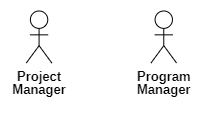
\includegraphics[width=0.3\columnwidth]{usecase/attori} 
    \caption{Attori}
\end{figure}
Gli attori che possiamo trovare all'interno dei casi d'uso rappresentano due risorse aziendali:
\subsubsection*{Project Manager}
Conosciuto come il "Responsabile di Progetto", si occupa dell'avvio, pianificazione ,esecuzione e controllo di un singolo progetto, seguendo tecniche di project management.\\
Le sue principali responsabilità sono:
\begin{itemize}
\item assicurarsi che i progetti siano allineati con gli obiettivi aziendali;
\item coordinare le risorse umane, assicurandosi che vengano utilizzate in modo efficiente;
\item stabilisce milestone, scadenze e obiettivi, monitorando lo stato di avanzamento dei progetti;
\item comunica con stakeholder, team di progetto e altre parti interessate.
\end{itemize}
\subsubsection*{Program Manager}
È un ruolo di gestione all'interno di un'organizzazione, ed è responsabile della pianificazione complessiva e del controllo di più progetti che compongono il suo programma. Collabora strettamente col Project Manager ed i loro compiti spesso si sovrappongono ma differiscono di portata, in quanto il Program Manager supervisiona gruppi di progetti gestiti singolarmente dai Project Manager.

\section{Casi d'uso}

\subsection{Scenario Anagrafiche}
\begin{figure}[H] 
    \centering 
    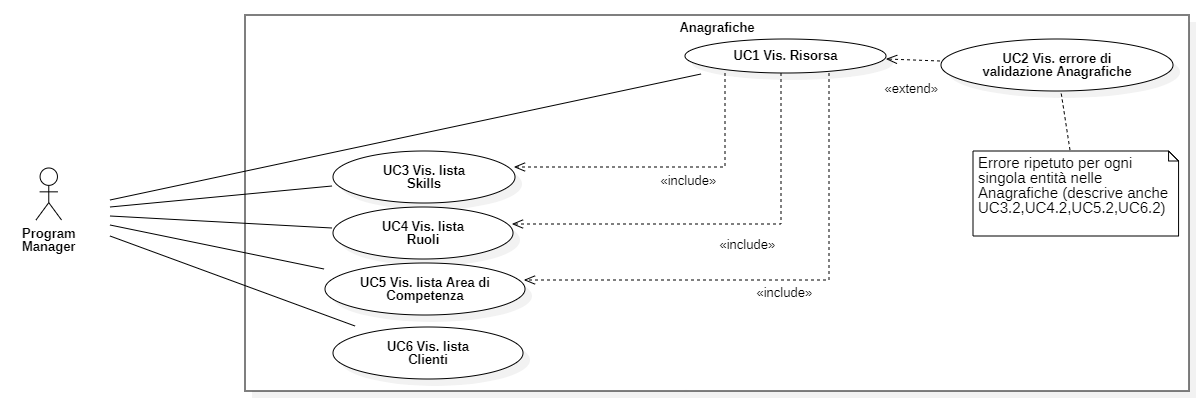
\includegraphics[width=1.1\columnwidth]{usecase/anagrafiche-general} 
    \caption{Casi d'Uso del scenario Anagrafiche}
\end{figure}

\subsubsection*{UC1 - Vis. Risorsa}

\begin{figure}[H] 
    \centering 
    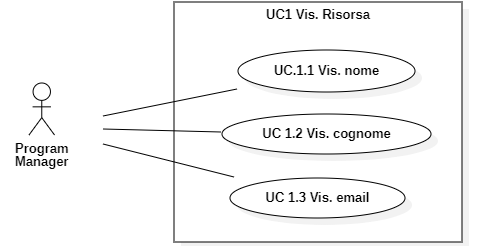
\includegraphics[width=0.6\columnwidth]{usecase/UC1} 
    \caption{Caso d'Uso 1 espanso}
\end{figure}

\begin{itemize}[label=$\circ$]
\item \textbf{Attore:} Program Manager;
\item \textbf{Descrizione:} il Program Manager può visualizzare una Risorsa;
\item \textbf{Precondizioni:} il richiedente è un Program Manager;
\item \textbf{Postcondizioni:} la Risorsa selezionata è visualizzabile dal Program Manager;
\item \textbf{Estensioni:} UC2;
\item \textbf{Inclusioni:} UC3, UC4, UC5.
\end{itemize}

\subsubsection*{UC1.1 - Vis. nome}
\begin{itemize}[label=$\circ$]
\item \textbf{Attore:} Program Manager;
\item \textbf{Descrizione:} il Program Manager può visualizzare il nome di una Risorsa;
\item \textbf{Precondizioni:} la Risorsa è visualizzabile dal Program Manager;
\item \textbf{Postcondizioni:} il Program Manager può visualizzare il nome della Risorsa selezionata;
\item \textbf{Estensioni:} il caso d'uso non ha estensioni;
\item \textbf{Inclusioni:} il caso d'uso non ha inclusioni.
\end{itemize}

\subsubsection*{UC1.2 - Vis. cognome}
\begin{itemize}[label=$\circ$]
\item \textbf{Attore:} Program Manager;
\item \textbf{Descrizione:} il Program Manager può visualizzare il cognome di una Risorsa;
\item \textbf{Precondizioni:}  la Risorsa è visualizzabile dal Program Manager;
\item \textbf{Postcondizioni:} il Program Manager può visualizzare il cognome della Risorsa selezionata;
\item \textbf{Estensioni:} il caso d'uso non ha estensioni;
\item \textbf{Inclusioni:} il caso d'uso non ha inclusioni.
\end{itemize}

\subsubsection*{UC1.3 - Vis. email}
\begin{itemize}[label=$\circ$]
\item \textbf{Attore:} Program Manager;
\item \textbf{Descrizione:} il Program Manager può visualizzare l'email di una Risorsa;
\item \textbf{Precondizioni:}  la Risorsa è visualizzabile dal Program Manager;
\item \textbf{Postcondizioni:} il Program Manager può visualizzare l'email della Risorsa selezionata;
\item \textbf{Estensioni:} il caso d'uso non ha estensioni;
\item \textbf{Inclusioni:} il caso d'uso non ha inclusioni.
\end{itemize}

\subsubsection*{UC2 - Vis. errore di validazione Anagrafiche}
\begin{itemize}[label=$\circ$]
\item \textbf{Attore:} Program Manager;
\item \textbf{Descrizione:} questo caso d'uso descrive anche UC3.2,UC4.2,UC5.2,UC6.2. Viene visualizzato un messaggio di errore in caso vengano eseguite funzionalità con dati non validi. Esso rappresenta errori di validazione nella richiesta fornita dall'utilizzatore;
\item \textbf{Precondizioni:} il Program Manager sta effettuando operazioni con dati non validi;
\item \textbf{Postcondizioni:} l'esecuzione della funzionalità è interrotta e viene visualizzato il messaggio di errore;
\item \textbf{Estensioni:} il caso d'uso non ha estensioni;
\item \textbf{Inclusioni:} il caso d'uso non ha inclusioni.
\end{itemize}

\subsubsection*{UC3 - Vis. lista Skill}
\begin{figure}[H] 
    \centering 
    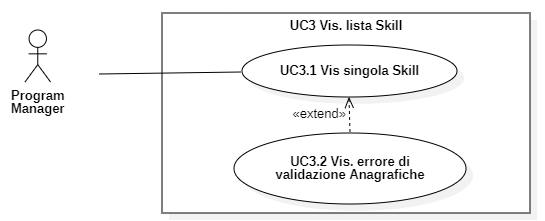
\includegraphics[width=0.6\columnwidth]{usecase/UC3} 
    \caption{Caso d'Uso 3 espanso}
\end{figure}
\begin{itemize}[label=$\circ$]
\item \textbf{Attore:} Program Manager;
\item \textbf{Descrizione:} il Program Manager può visualizzare la lista delle Skill;
\item \textbf{Precondizioni:} il richiedente è un Program Manager;
\item \textbf{Postcondizioni:} la lista delle Skill è visualizzabile dal Program Manager;
\item \textbf{Estensioni:} il caso d'uso non ha estensioni;
\item \textbf{Inclusioni:} il caso d'uso non ha inclusioni.
\end{itemize}

\subsubsection*{UC3.1 - Vis. singola Skill}
\begin{figure}[H] 
    \centering 
    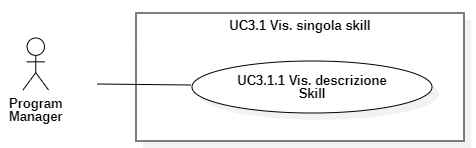
\includegraphics[width=0.6\columnwidth]{usecase/UC3.1} 
    \caption{Caso d'Uso 3.1 espanso}
\end{figure}
\begin{itemize}[label=$\circ$]
\item \textbf{Attore:} Program Manager;
\item \textbf{Descrizione:} il Program Manager può visualizzare una Skill;
\item \textbf{Precondizioni:} il richiedente è un Program Manager;
\item \textbf{Postcondizioni:} la Skill selezionata è visualizzabile dal Program Manager;
\item \textbf{Estensioni:} UC3.2;
\item \textbf{Inclusioni:} il caso d'uso non ha inclusioni.
\end{itemize}

\subsubsection*{UC3.1.1 - Vis. descrizione Skill}
\begin{itemize}[label=$\circ$]
\item \textbf{Attore:} Program Manager;
\item \textbf{Descrizione:} il Program Manager può visualizzare la descrizione di una Skill;
\item \textbf{Precondizioni:} la Skill è visualizzabile dal Program Manager;
\item \textbf{Postcondizioni:} il Program Manager può visualizzare la descrizione della Skill selezionata;
\item \textbf{Estensioni:} il caso d'uso non ha estensioni;
\item \textbf{Inclusioni:} il caso d'uso non ha inclusioni.
\end{itemize}

\subsubsection*{UC4 - Vis. lista Ruoli}
\begin{figure}[H] 
    \centering 
    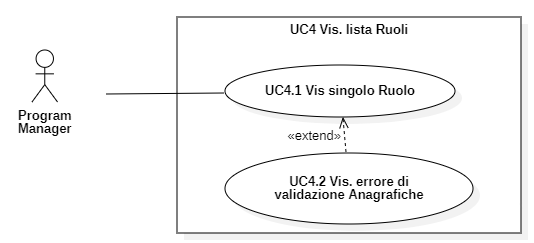
\includegraphics[width=0.6\columnwidth]{usecase/UC4} 
    \caption{Caso d'Uso 4 espanso}
\end{figure}
\begin{itemize}[label=$\circ$]
\item \textbf{Attore:} Program Manager;
\item \textbf{Descrizione:} il Program Manager può visualizzare la lista dei Ruoli;
\item \textbf{Precondizioni:} il richiedente è un Program Manager;
\item \textbf{Postcondizioni:} la lista dei Ruoli è visualizzabile dal Program Manager;
\item \textbf{Estensioni:} il caso d'uso non ha estensioni;
\item \textbf{Inclusioni:} il caso d'uso non ha inclusioni.
\end{itemize}

\subsubsection*{UC4.1 - Vis. singolo Ruolo}
\begin{figure}[H] 
    \centering 
    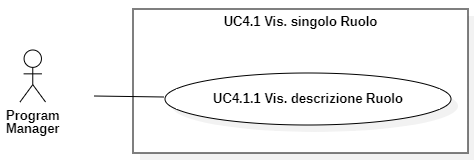
\includegraphics[width=0.6\columnwidth]{usecase/UC4.1} 
    \caption{Caso d'Uso 4.1 espanso}
\end{figure}
\begin{itemize}[label=$\circ$]
\item \textbf{Attore:} Program Manager;
\item \textbf{Descrizione:} il Program Manager può visualizzare un Ruolo;
\item \textbf{Precondizioni:} il richiedente è un Program Manager;
\item \textbf{Postcondizioni:} il Ruolo selezionato è visualizzabile dal Program Manager;
\item \textbf{Estensioni:}  UC4.2;
\item \textbf{Inclusioni:} il caso d'uso non ha inclusioni.
\end{itemize}

\subsubsection*{UC4.1.1 - Vis. descrizione Ruolo}
\begin{itemize}[label=$\circ$]
\item \textbf{Attore:} Program Manager;
\item \textbf{Descrizione:} il Program Manager può visualizzare la descrizione di un Ruolo;
\item \textbf{Precondizioni:}  il Ruolo è visualizzabile dal Program Manager;
\item \textbf{Postcondizioni:} il Program Manager può visualizzare la descrizione del Ruolo selezionato;
\item \textbf{Estensioni:} il caso d'uso non ha estensioni;
\item \textbf{Inclusioni:} il caso d'uso non ha inclusioni.
\end{itemize}

\subsubsection*{UC5 - Vis. lista Area di Competenza}
\begin{figure}[H] 
    \centering 
    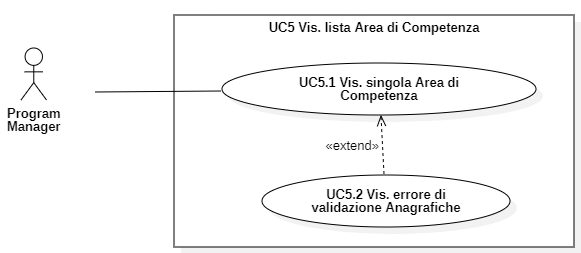
\includegraphics[width=0.6\columnwidth]{usecase/UC5} 
    \caption{Caso d'Uso 5 espanso}
\end{figure}
\begin{itemize}[label=$\circ$]
\item \textbf{Attore:} Program Manager;
\item \textbf{Descrizione:} il Program Manager può visualizzare la lista delle Aree di Competenza;
\item \textbf{Precondizioni:} il richiedente è un Program Manager;
\item \textbf{Postcondizioni:} la lista delle Aree di Competenza è visualizzabile dal Program Manager;
\item \textbf{Estensioni:} il caso d'uso non ha estensioni;
\item \textbf{Inclusioni:} il caso d'uso non ha inclusioni.
\end{itemize}

\subsubsection*{UC5.1 - Vis. singola Area di Competenza}
\begin{figure}[H] 
    \centering 
    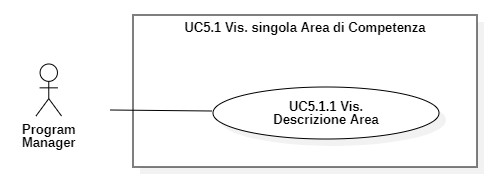
\includegraphics[width=0.6\columnwidth]{usecase/UC5.1} 
    \caption{Caso d'Uso 5.1 espanso}
\end{figure}
\begin{itemize}[label=$\circ$]
\item \textbf{Attore:} Program Manager;
\item \textbf{Descrizione:} il Program Manager può visualizzare un'Area di Competenza;
\item \textbf{Precondizioni:} il richiedente è un Program Manager;
\item \textbf{Postcondizioni:} l'Area di Competenza selezionata è visualizzabile dal Program Manager;
\item \textbf{Estensioni:}  UC5.2;
\item \textbf{Inclusioni:} il caso d'uso non ha inclusioni.
\end{itemize}

\subsubsection*{UC5.1.1 - Vis. descrizione Area}
\begin{itemize}[label=$\circ$]
\item \textbf{Attore:} Program Manager;
\item \textbf{Descrizione:} il Program Manager può visualizzare la descrizione di un'Area di Competenza;
\item \textbf{Precondizioni:}  l'Area è visualizzabile dal Program Manager;
\item \textbf{Postcondizioni:} il Program Manager può visualizzare la descrizione dell'Area di Competenza selezionata;
\item \textbf{Estensioni:} non ci sono estensioni;
\item \textbf{Inclusioni:} non ci sono inclusioni.
\end{itemize}

\subsubsection*{UC6 - Vis. lista Clienti}
\begin{figure}[H] 
    \centering 
    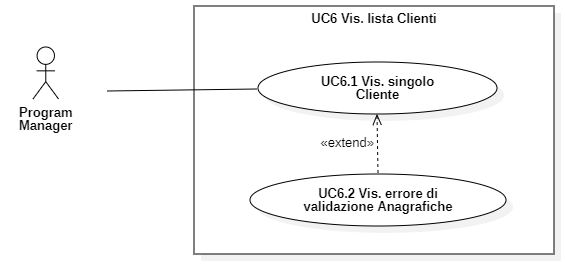
\includegraphics[width=0.6\columnwidth]{usecase/UC6} 
    \caption{Caso d'Uso 6 espanso}
\end{figure}
\begin{itemize}[label=$\circ$]
\item \textbf{Attore:} Program Manager;
\item \textbf{Descrizione:} il Program Manager può visualizzare la lista dei Clienti;
\item \textbf{Precondizioni:} il richiedente è un Program Manager;
\item \textbf{Postcondizioni:} la lista dei Clienti è visualizzabile dal Program Manager;
\item \textbf{Estensioni:} il caso d'uso non ha estensioni;
\item \textbf{Inclusioni:} il caso d'uso non ha inclusioni.
\end{itemize}

\subsubsection*{UC6.1 - Vis. singolo Cliente}
\begin{figure}[H] 
    \centering 
    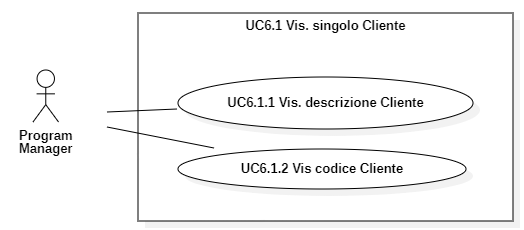
\includegraphics[width=0.6\columnwidth]{usecase/UC6.1} 
    \caption{Caso d'Uso 6.1 espanso}
\end{figure}
\begin{itemize}[label=$\circ$]
\item \textbf{Attore:} Program Manager;
\item \textbf{Descrizione:} il Program Manager può visualizzare un Cliente;
\item \textbf{Precondizioni:} il richiedente è un Program Manager;
\item \textbf{Postcondizioni:} il Cliente selezionato è visualizzabile dal Program Manager;
\item \textbf{Estensioni:} UC6.2;
\item \textbf{Inclusioni:} non ci sono inclusioni.
\end{itemize}

\subsubsection*{UC6.1.1 - Vis. descrizione Cliente}
\begin{itemize}[label=$\circ$]
\item \textbf{Attore:} Program Manager;
\item \textbf{Descrizione:} il Program Manager può visualizzare la descrizione di Cliente;
\item \textbf{Precondizioni:}  il Cliente è visualizzabile dal Program Manager;
\item \textbf{Postcondizioni:} il Program Manager può visualizzare la descrizione del Cliente selezionato;
\item \textbf{Estensioni:} il caso d'uso non ha estensioni;
\item \textbf{Inclusioni:} il caso d'uso non ha inclusioni.
\end{itemize}

\subsubsection*{UC6.1.2 - Vis. codice Cliente}
\begin{itemize}[label=$\circ$]
\item \textbf{Attore:} Program Manager;
\item \textbf{Descrizione:} il Program Manager può visualizzare il codice del Cliente;
\item \textbf{Precondizioni:} il Cliente è visualizzabile dal Program Manager;
\item \textbf{Postcondizioni:} il Program Manager può visualizzare il codice del Cliente selezionato;
\item \textbf{Estensioni:} il caso d'uso non ha estensioni;
\item \textbf{Inclusioni:} il caso d'uso non ha inclusioni.
\end{itemize}


\subsection{Scenario Richieste}
\begin{figure}[H] 
    \centering 
    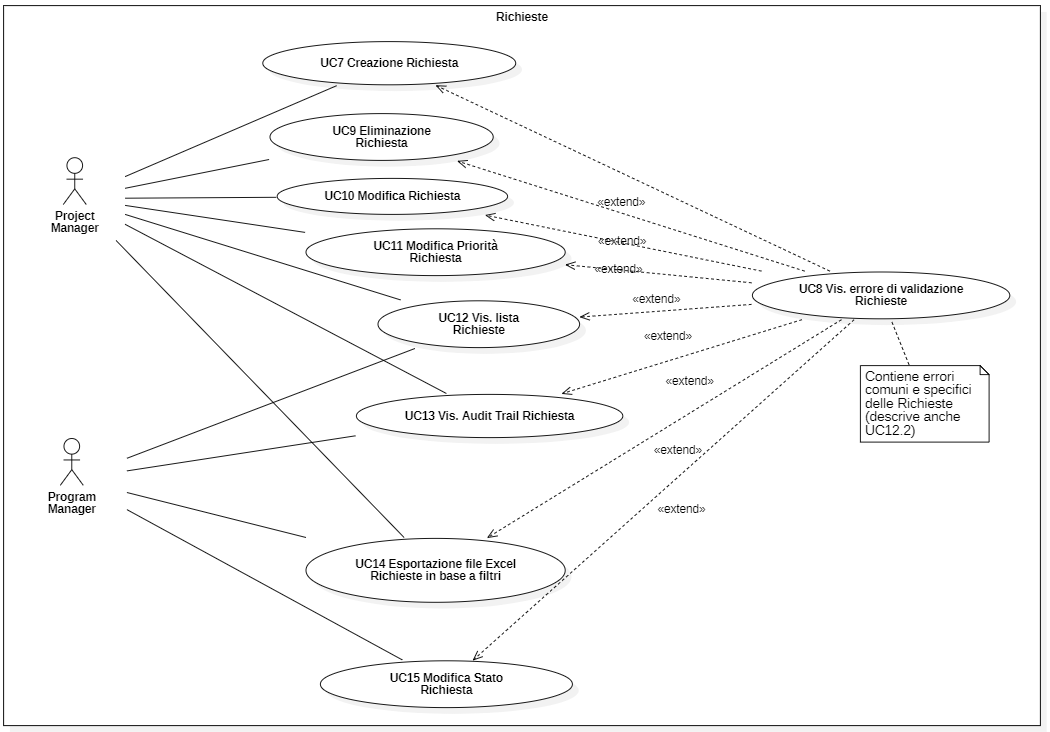
\includegraphics[width=1.1\columnwidth]{usecase/richieste-general} 
    \caption{Casi d'Uso del scenario Richieste}
\end{figure}

\subsubsection*{UC7 - Creazione Richiesta}
\begin{itemize}[label=$\circ$]
\item \textbf{Attore:} Project Manager;
\item \textbf{Descrizione:} il Project Manager può creare una nuova Richiesta;
\item \textbf{Precondizioni:} il richiedente è un Project Manager;
\item \textbf{Postcondizioni:} la Richiesta è stata creata dal Project Manager con successo;
\item \textbf{Estensioni:} UC8;
\item \textbf{Inclusioni:} il caso d'uso non ha inclusioni.
\end{itemize}

\subsubsection*{UC8 - Vis. errore di validazione Richieste}
\begin{itemize}[label=$\circ$]
\item \textbf{Attore:} Project Manager e Program Manager;
\item \textbf{Descrizione:}  questo caso d'uso descrive anche UC12.2. Viene visualizzato un messaggio di errore in caso vengano eseguite funzionalità con dati non validi. Esso rappresenta i seguenti errori comuni all'interno delle Richieste: dati non validi, filtri non valorizzati, entità associate non valide, risultati nulli o non valorizzati;
\item \textbf{Precondizioni:} il Program Manger o il Project Manager stanno effettuando operazioni con dati non validi;
\item \textbf{Postcondizioni:} l'esecuzione della funzionalità è interrotta e viene visualizzato il messaggio di errore;
\item \textbf{Estensioni:} il caso d'uso non ha estensioni;
\item \textbf{Inclusioni:} il caso d'uso non ha inclusioni.
\end{itemize}

\subsubsection*{UC9 - Eliminazione Richiesta}
\begin{itemize}[label=$\circ$]
\item \textbf{Attore:} Project Manager;
\item \textbf{Descrizione:} il Project Manager può eliminare una Richiesta esistente;
\item \textbf{Precondizioni:} il richiedente è un Project Manager;
\item \textbf{Postcondizioni:} la Richiesta è stata eliminata dal Project Manager con successo;
\item \textbf{Estensioni:} UC8;
\item \textbf{Inclusioni:} il caso d'uso non ha inclusioni.
\end{itemize}

\subsubsection*{UC10 - Modifica Richiesta}
\begin{itemize}[label=$\circ$]
\item \textbf{Attore:} Project Manager;
\item \textbf{Descrizione:} il Project Manager può modificare una Richiesta esistente nella sua totalità sovrascrivendola;
\item \textbf{Precondizioni:} il richiedente è un Project Manager;
\item \textbf{Postcondizioni:} la Richiesta selezionata è stata modificata con successo;
\item \textbf{Estensioni:} UC8;
\item \textbf{Inclusioni:} il caso d'uso non ha inclusioni.
\end{itemize}

\subsubsection*{UC11 - Modifica Priorità Richiesta}
\begin{itemize}[label=$\circ$]
\item \textbf{Attore:} Project Manager;
\item \textbf{Descrizione:} il Project Manager può modificare l'attributo Priorità di una Richiesta esistente inserendo un valore tra: Alta, Media o Bassa;
\item \textbf{Precondizioni:} il richiedente è un Project Manager;
\item \textbf{Postcondizioni:} la Richiesta è stata modificata con successo solo nel campo Priorità dal Project Manager;
\item \textbf{Estensioni:} UC8;
\item \textbf{Inclusioni:} il caso d'uso non ha inclusioni.
\end{itemize}

\subsubsection*{UC12 - Vis. lista Richieste}

\begin{figure}[H] 
    \centering 
    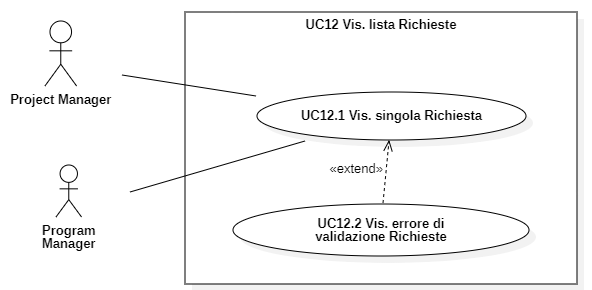
\includegraphics[width=0.6\columnwidth]{usecase/UC12} 
    \caption{Caso d'Uso 12 espanso}
\end{figure}

\begin{itemize}[label=$\circ$]
\item \textbf{Attore:} Project Manager e Program Manager;
\item \textbf{Descrizione:} il Project Manager e il Program Manager possono visualizzare una lista di Richieste dopo aver inserito filtri e/o una parola nella ricerca rapida e aver selezionato se i filtri applicati devono essere congiunti o disgiunti;
\item \textbf{Precondizioni:} il richiedente è un Project Manager o un Program Manager;
\item \textbf{Postcondizioni:} la lista delle Richieste è visualizzabile dal Project Manager e dal Program Manager;
\item \textbf{Estensioni:} UC8;
\item \textbf{Inclusioni:} il caso d'uso non ha inclusioni.
\end{itemize}

\subsubsection*{UC12.1 - Vis. singola Richiesta}

\begin{figure}[H] 
    \centering 
    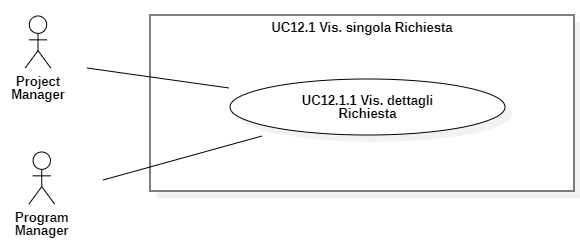
\includegraphics[width=0.6\columnwidth]{usecase/UC12.1} 
    \caption{Caso d'Uso 12.1 espanso}
\end{figure}

\begin{itemize}[label=$\circ$]
\item \textbf{Attore:} Project Manager e Program Manager;
\item \textbf{Descrizione:} il Project Manager e il Program Manager possono visualizzare la Richiesta selezionata;
\item \textbf{Precondizioni:} la lista delle Richieste è visualizzabile;
\item \textbf{Postcondizioni:} la Richiesta selezionata è visualizzabile dal Program Manager e dal Project Manager;
\item \textbf{Estensioni:} UC12.2;
\item \textbf{Inclusioni:} il caso d'uso non ha inclusioni.
\end{itemize}

\subsubsection*{UC12.1.1 - Vis. dettagli Richiesta}

\begin{figure}[H] 
    \centering 
    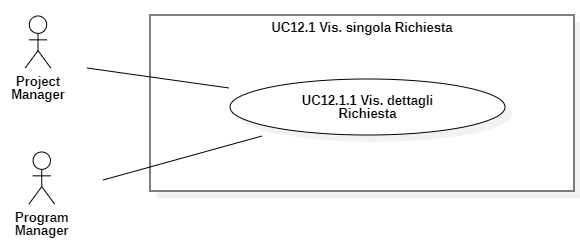
\includegraphics[width=0.6\columnwidth]{usecase/UC12.1} 
    \caption{Caso d'Uso 12.1 espanso}
\end{figure}

\begin{itemize}[label=$\circ$]
\item \textbf{Attore:} Project Manager e Program Manager;
\item \textbf{Descrizione:} il Project Manager e il Program Manager possono visualizzare la Richiesta selezionata;
\item \textbf{Precondizioni:} la Richiesta singola è visualizzabile;
\item \textbf{Postcondizioni:} il Project Manager e il Program Manager possono visualizzare i campi di una Richiesta selezionata;
\item \textbf{Estensioni:} il caso d'uso non ha esclusioni;
\item \textbf{Inclusioni:} il caso d'uso non ha inclusioni.
\end{itemize}

\subsubsection*{UC13 - Vis. audit trail Richiesta}

\begin{figure}[H] 
    \centering 
    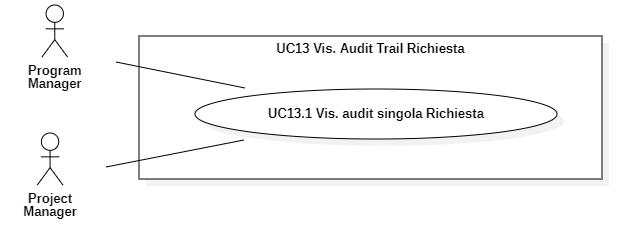
\includegraphics[width=0.6\columnwidth]{usecase/UC13} 
    \caption{Caso d'Uso 13 espanso}
\end{figure}

\begin{itemize}[label=$\circ$]
\item \textbf{Attore:} Project Manager e Program Manager;
\item \textbf{Descrizione:} il Project Manager e il Program Manager possono visualizzare l'audit trail di una Richiesta selezionata.;
\item \textbf{Precondizioni:} il richiedente è un Project Manager o un Program Manager;
\item \textbf{Postcondizioni:} la traccia di audit della Richiesta selezionata è visualizzabile dal Project Manager e dal Program Manager;
\item \textbf{Estensioni:} UC8;
\item \textbf{Inclusioni:} il caso d'uso non ha inclusioni.
\end{itemize}

\subsubsection*{UC13.1 - Vis. audit singola Richiesta}

\begin{figure}[H] 
    \centering 
    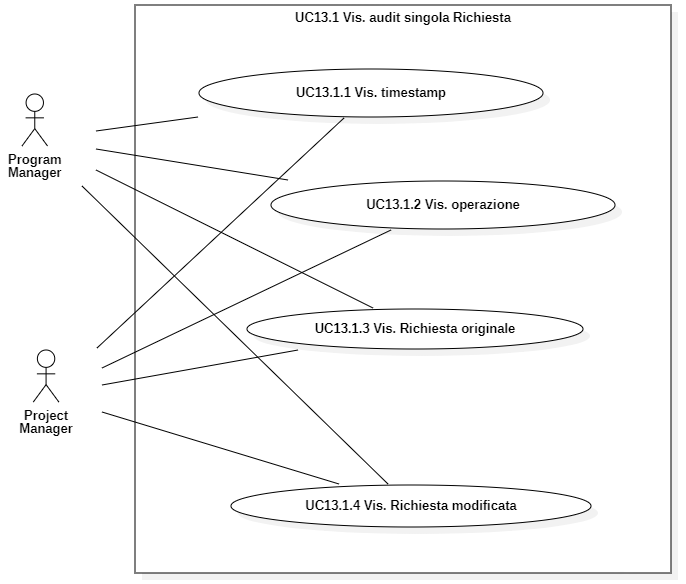
\includegraphics[width=0.8\columnwidth]{usecase/UC13.1} 
    \caption{Caso d'Uso 13.1 espanso}
\end{figure}

\begin{itemize}[label=$\circ$]
\item \textbf{Attore:} Project Manager e Program Manager;
\item \textbf{Descrizione:} il Project Manager e il Program Manager possono visualizzare l'audit di una singola Richiesta;
\item \textbf{Precondizioni:} l'audit trail è visualizzabile;
\item \textbf{Postcondizioni:} l'audit di una singola Richiesta è visualizzabile;
\item \textbf{Estensioni:} il caso d'uso non ha estensioni;
\item \textbf{Inclusioni:} il caso d'uso non ha inclusioni.
\end{itemize}

\subsubsection*{UC13.1.1 - Vis. timestamp}
\begin{itemize}[label=$\circ$]
\item \textbf{Attore:} Project Manager e Program Manager;
\item \textbf{Descrizione:} il Project Manager e il Program Manager possono visualizzare il timestamp di una singola audit di una Richiesta;
\item \textbf{Precondizioni:} la singola audit di una Richiesta è visualizzabile;
\item \textbf{Postcondizioni:} il timestamp della singola audit è visualizzabile;
\item \textbf{Estensioni:} il caso d'uso non ha estensioni;
\item \textbf{Inclusioni:} il caso d'uso non ha inclusioni.
\end{itemize}

\subsubsection*{UC13.1.2 - Vis. operazione}
\begin{itemize}[label=$\circ$]
\item \textbf{Attore:} Project Manager e Program Manager;
\item \textbf{Descrizione:} il Project Manager e il Program Manager possono visualizzare l'operazione di una singola audit di una Richiesta;
\item \textbf{Precondizioni:} la singola audit di una Richiesta è visualizzabile;
\item \textbf{Postcondizioni:} l'operazione della singola audit è visualizzabile;
\item \textbf{Estensioni:} il caso d'uso non ha estensioni;
\item \textbf{Inclusioni:} il caso d'uso non ha inclusioni.
\end{itemize}

\subsubsection*{UC13.1.3 - Vis. Richiesta originale}
\begin{itemize}[label=$\circ$]
\item \textbf{Attore:} Project Manager e Program Manager;
\item \textbf{Descrizione:} il Project Manager e il Program Manager possono visualizzare la singola audit di una Richiesta prima che l'operazione venga eseguita;
\item \textbf{Precondizioni:} la singola audit di una Richiesta è visualizzabile;
\item \textbf{Postcondizioni:} la Richiesta originale della singola audit è visualizzabile;
\item \textbf{Estensioni:} il caso d'uso non ha estensioni;
\item \textbf{Inclusioni:} il caso d'uso non ha inclusioni.
\end{itemize}

\subsubsection*{UC13.1.4 - Vis. Richiesta modificata}
\begin{itemize}[label=$\circ$]
\item \textbf{Attore:} Project Manager e Program Manager;
\item \textbf{Descrizione:} il Project Manager e il Program Manager possono visualizzare la singola audit di una Richiesta dopo che l'operazione è stata eseguita;
\item \textbf{Precondizioni:} la singola audit di una Richiesta è visualizzabile;
\item \textbf{Postcondizioni:} la Richiesta modificata della singola audit è visualizzabile;
\item \textbf{Estensioni:} il caso d'uso non ha estensioni;
\item \textbf{Inclusioni:} il caso d'uso non ha inclusioni.
\end{itemize}

\subsubsection*{UC14 - Esportazione file Excel Richieste in base a filtri}
\begin{itemize}[label=$\circ$]
\item \textbf{Attore:} Project Manager e Program Manager;
\item \textbf{Descrizione:} il Project Manager e il Program Manager possono esportare in un file Excel scaricabile un report delle Richieste in base a dei filtri inseriti;
\item \textbf{Precondizioni:} il richiedente è un Project Manager o un Program Manager;
\item \textbf{Postcondizioni:} il report Excel è stato generato correttamente ed è possibile scaricarlo;
\item \textbf{Estensioni:} UC8;
\item \textbf{Inclusioni:} il caso d'uso non ha inclusioni.
\end{itemize}

\subsubsection*{UC15 - Modifica Stato Richiesta}
\begin{itemize}[label=$\circ$]
\item \textbf{Attore:} Program Manager;
\item \textbf{Descrizione:} il Program Manager può cambiare lo stato di una Richiesta esistente impostandolo in uno dei seguenti valori: Evasa, Non Evasa, Aperta, In corso, Chiusa;
\item \textbf{Precondizioni:} il richiedente è un Program Manager;
\item \textbf{Postcondizioni:} solo lo stato della Richiesta è stato modificato con successo;
\item \textbf{Estensioni:} UC8;
\item \textbf{Inclusioni:} il caso d'uso non ha inclusioni.
\end{itemize}



\subsection{Scenario Pianificazioni}
\begin{figure}[H] 
    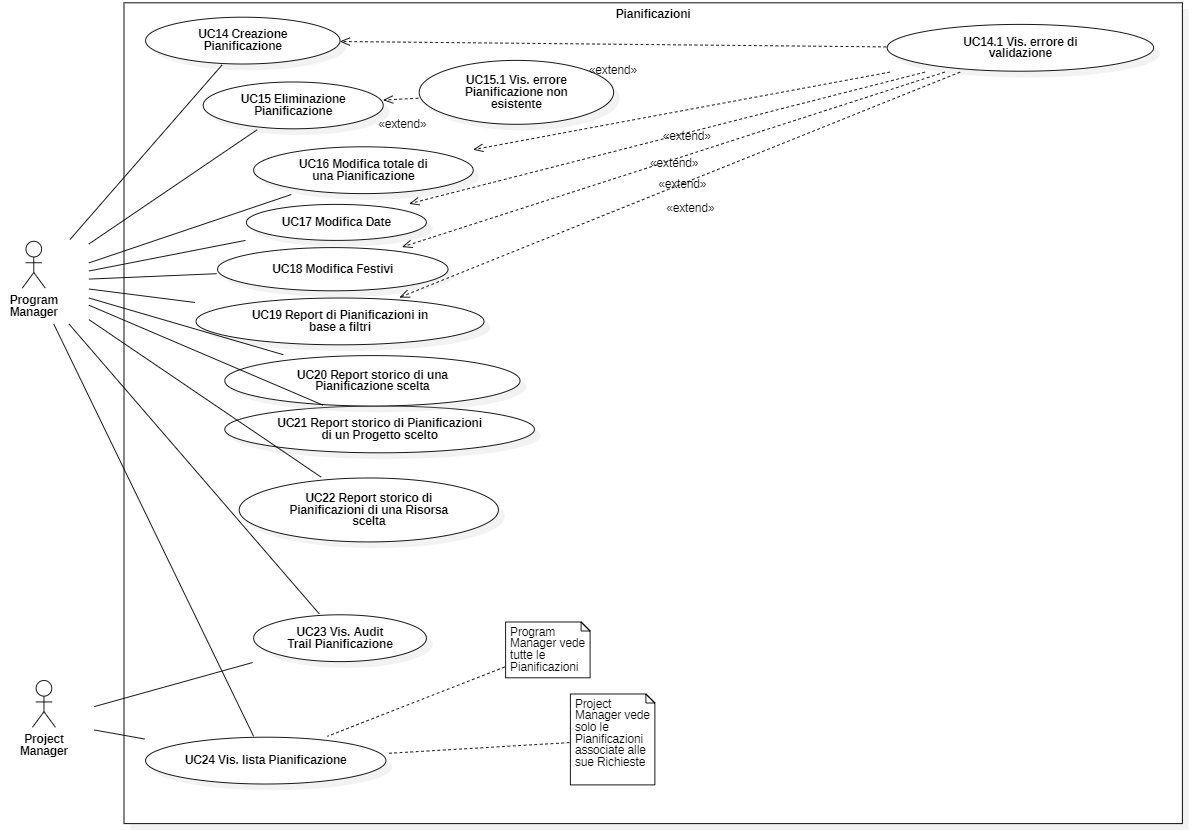
\includegraphics[width=1.00\linewidth]{usecase/pianificazioni-general} 
    \caption{Casi d'Uso del scenario Pianificazioni}
\end{figure}

\subsubsection*{UC16 - Creazione Pianificazione}
\begin{itemize}[label=$\circ$]
\item \textbf{Attore:} Program Manager;
\item \textbf{Descrizione:} il Program Manager può creare una Pianificazione per Figura richiesta da una Richiesta;
\item \textbf{Precondizioni:} il richiedente è un Program Manager;
\item \textbf{Postcondizioni:} la Pianificazione è stata creata dal Program Manager con successo;
\item \textbf{Estensioni:} UC17;
\item \textbf{Inclusioni:} il caso d'uso non ha inclusioni.
\end{itemize}

\subsubsection*{UC17 - Vis. errore di validazione Pianificazioni}
\begin{itemize}[label=$\circ$]
\item \textbf{Attore:} Project Manager e Program Manager;
\item \textbf{Descrizione:} questo caso d'uso descrive anche UC26.2. Viene visualizzato un messaggio di errore in caso vengano eseguite funzionalità con dati non validi. Esso rappresenta i seguenti errori comuni all'interno delle Pianificazioni: dati non validi, filtri non valorizzati, entità associate non valide, risultati nulli o non valorizzati;
\item \textbf{Precondizioni:} il Program Manager o il Project Manager stanno effettuando operazioni con dati non validi;
\item \textbf{Postcondizioni:} l'esecuzione della funzionalità è interrotta e viene visualizzato il messaggio di errore;
\item \textbf{Estensioni:} il caso d'uso non ha estensioni;
\item \textbf{Inclusioni:} il caso d'uso non ha inclusioni.
\end{itemize}

\subsubsection*{UC18 - Eliminazione Pianificazione}
\begin{itemize}[label=$\circ$]
\item \textbf{Attore:} Program Manager;
\item \textbf{Descrizione:} il Program Manager può eliminare una Pianificazione esistente;
\item \textbf{Precondizioni:} il richiedente è il Program Manager;
\item \textbf{Postcondizioni:} la Pianificazione è stata eliminata dal Program Manager con successo;
\item \textbf{Estensioni:} UC17;
\item \textbf{Inclusioni:} il caso d'uso non ha inclusioni.
\end{itemize}

\subsubsection*{UC19 - Modifica Pianificazione}
\begin{itemize}[label=$\circ$]
\item \textbf{Attore:} Program Manager;
\item \textbf{Descrizione:} il Program Manager può modificare una Pianificazione esistente nella sua totalità sovrascrivendola;
\item \textbf{Precondizioni:} il richiedente è un Program Manager;
\item \textbf{Postcondizioni:} la Pianificazione selezionata è stata modificata con successo;
\item \textbf{Estensioni:} UC17;
\item \textbf{Inclusioni:} il caso d'uso non ha inclusioni.
\end{itemize}

\subsubsection*{UC20 - Modifica Date}
\begin{itemize}[label=$\circ$]
\item \textbf{Attore:} Program Manager;
\item \textbf{Descrizione:} il Program Manager può modificare le date di inizio e/o di fine di una Pianificazione;
\item \textbf{Precondizioni:} il richiedente è un Program Manager;
\item \textbf{Postcondizioni:} la Pianificazione è stata modificata con successo solo nel campo Data inizio e/o Data fine dal Program Manager;
\item \textbf{Estensioni:} UC17;
\item \textbf{Inclusioni:} il caso d'uso non ha inclusioni.
\end{itemize}

\subsubsection*{UC21 - Modifica Festivi}
\begin{itemize}[label=$\circ$]
\item \textbf{Attore:} Program Manager;
\item \textbf{Descrizione:} il Porgram Manager può modificare il campo Festivi di una Pianificazione. Se posto a vero il lavoratore potrà lavorare anche nei giorni festivi;
\item \textbf{Precondizioni:} il richiedente è un Program Manager;
\item \textbf{Postcondizioni:}  la Pianificazione è stata modificata con successo solo nel campo Festivi dal Program Manager;
\item \textbf{Estensioni:} UC17;
\item \textbf{Inclusioni:} il caso d'uso non ha inclusioni.
\end{itemize}

\subsubsection*{UC22 - Esportazione file Excel di Pianificazioni in base a filtri}
\begin{itemize}[label=$\circ$]
\item \textbf{Attore:} Program Manager;
\item \textbf{Descrizione:} : il Program Manager può esportare in un
file Excel scaricabile un report delle Pianificazioni in base a dei filtri inseriti;
\item \textbf{Precondizioni:} : il richiedente è un Program Manager;
\item \textbf{Postcondizioni:} il report Excel è stato generato correttamente ed è possibile
scaricarlo;
\item \textbf{Estensioni:} UC17;
\item \textbf{Inclusioni:} il caso d'uso non ha inclusioni.
\end{itemize}

\subsubsection*{UC23 - Esportazione storico Excel di Pianificazioni di un Progetto}
\begin{itemize}[label=$\circ$]
\item \textbf{Attore:} Program Manager;
\item \textbf{Descrizione:} il Program Manager può esportare in un file Excel scaricabile uno storico di Pianificazioni associate ad un Progetto contenente tutte le risorse allocate e l’effettivo impiego di queste nelle attività;
\item \textbf{Precondizioni:} il richiedente è un Program Manager;
\item \textbf{Postcondizioni:} il report Excel è stato generato correttamente ed è possibile
scaricarlo;
\item \textbf{Estensioni:} UC17;
\item \textbf{Inclusioni:} il caso d'uso non ha inclusioni.
\end{itemize}

\subsubsection*{UC24 - Esportazione storico Excel di Pianificazioni di una Risorsa}
\begin{itemize}[label=$\circ$]
\item \textbf{Attore:} Program Manager;
\item \textbf{Descrizione:} il Program Manager può esportare in un file Excel scaricabile uno storico di Pianificazioni in cui c'è stata una determinata Risorsa;
\item \textbf{Precondizioni:} il richiedente è un Program Manager;
\item \textbf{Postcondizioni:} il report Excel è stato generato correttamente ed è possibile
scaricarlo;
\item \textbf{Estensioni:} UC17;
\item \textbf{Inclusioni:} il caso d'uso non ha inclusioni.
\end{itemize}

\subsubsection*{UC25 - Vis. Audit Trail Pianificazione}
\begin{figure}[H] 
    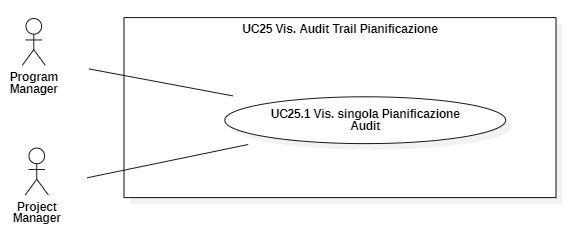
\includegraphics[width=0.65\linewidth]{usecase/UC25} 
    \caption{Caso d'Uso 25 espanso}
\end{figure}

\begin{itemize}[label=$\circ$]
\item \textbf{Attore:} Project Manager o Program Manager;
\item \textbf{Descrizione:} il Project Manager o il Program Manager possono visualizzare
l’audit trail di una Richiesta selezionata. Il Project Manager può vedere solo le tracce di audit delle Pianificazioni associate alle sue Richieste, mentre il Program Manager può vederle tutte;
\item \textbf{Precondizioni:} il richiedente è un Program Manager o un Project Manager;
\item \textbf{Postcondizioni:} la traccia di audit della Pianificazione selezionata è visualizzabile dal Project Manager o dal Program Manager;
\item \textbf{Estensioni:} UC17;
\item \textbf{Inclusioni:} il caso d'uso non ha inclusioni.
\end{itemize}


\subsubsection*{UC25.1 - Vis. singola Pianificazione Audit}
\begin{figure}[H] 
    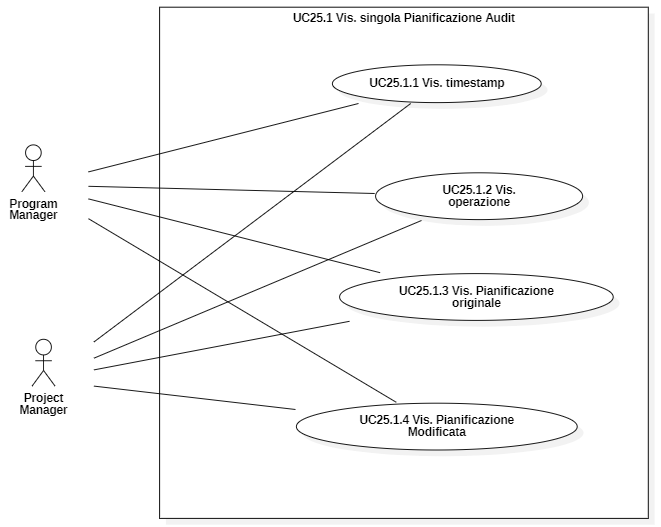
\includegraphics[width=0.75\linewidth]{usecase/UC25.1} 
    \caption{Caso d'Uso 25.1 espanso}
\end{figure}

\begin{itemize}[label=$\circ$]
\item \textbf{Attore:} Project Manager o Program Manager;
\item \textbf{Descrizione:} il Project Manager o il Program Manager può vedere l'audit di una singola Pianificazione. Il Project Manager può vedere solo le Pianificazioni associate alle sue Richieste, mentre il Program Manager può vederle tutte;
\item \textbf{Precondizioni:} l'audit trail è visualizzabile;
\item \textbf{Postcondizioni:} l'audit di una singola Pianificazione è visualizzabile;
\item \textbf{Estensioni:} il caso d'uso non ha estensioni;
\item \textbf{Inclusioni:} il caso d'uso non ha inclusioni.
\end{itemize}

\subsubsection*{UC25.1.1 - Vis. timestamp}

\begin{itemize}[label=$\circ$]
\item \textbf{Attore:} Project Manager o Program Manager;
\item \textbf{Descrizione:} il Project Manager e il Program Manager possono visualizzare il
timestamp di una singola audit di una Pianificazione;
\item \textbf{Precondizioni:} la singola audit di una Pianificazione è visualizzabile;
\item \textbf{Postcondizioni:} il timestamp della singola audit è visualizzabile;
\item \textbf{Estensioni:} il caso d'uso non ha estensioni;
\item \textbf{Inclusioni:} il caso d'uso non ha inclusioni.
\end{itemize}

\subsubsection*{UC25.1.2 - Vis. operazione}

\begin{itemize}[label=$\circ$]
\item \textbf{Attore:} Project Manager o Program Manager;
\item \textbf{Descrizione:} il Project Manager e il Program Manager possono visualizzare l'operazione di una singola audit di una Pianificazione;
\item \textbf{Precondizioni:} la singola audit di una Pianificazione è visualizzabile;
\item \textbf{Postcondizioni:} l’operazione della singola audit è visualizzabile;
\item \textbf{Estensioni:} il caso d'uso non ha estensioni;
\item \textbf{Inclusioni:} il caso d'uso non ha inclusioni.
\end{itemize}

\subsubsection*{UC25.1.3 - Vis. Pianificazione originale}

\begin{itemize}[label=$\circ$]
\item \textbf{Attore:} Project Manager o Program Manager;
\item \textbf{Descrizione:} il Project Manager o il Program Manager possono visualizzare la
singola audit di una Pianificazione prima che l’operazione venga eseguita;
\item \textbf{Precondizioni:}la singola audit di una Pianificazione è visualizzabile;
\item \textbf{Postcondizioni:} la Richiesta originale della singola audit è visualizzabile;
\item \textbf{Estensioni:} il caso d'uso non ha estensioni;
\item \textbf{Inclusioni:} il caso d'uso non ha inclusioni.
\end{itemize}

\subsubsection*{UC25.1.4 - Vis. Pianificazione modificata}

\begin{itemize}[label=$\circ$]
\item \textbf{Attore:} Project Manager o Program Manager;
\item \textbf{Descrizione:} il Project Manager o il Program Manager possono visualizzare la
singola audit di una Pianificazione dopo che l’operazione è stata eseguita;
\item \textbf{Precondizioni:} la singola audit di una Pianificazione è visualizzabile;
\item \textbf{Postcondizioni:} la Pianificazione modificata della singola audit è visualizzabile;
\item \textbf{Estensioni:} il caso d'uso non ha estensioni;
\item \textbf{Inclusioni:} il caso d'uso non ha inclusioni.
\end{itemize}

\subsubsection*{UC26 - Vis. lista Pianificazione}
\begin{figure}[H] 
    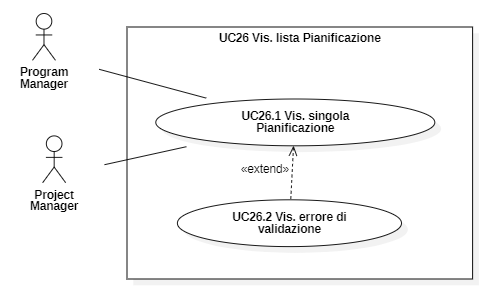
\includegraphics[width=0.65\linewidth]{usecase/UC26} 
    \caption{Caso d'Uso 26 espanso}
\end{figure}

\begin{itemize}[label=$\circ$]
\item \textbf{Attore:}  Project Manager o Program Manager;
\item \textbf{Descrizione:} il Project Manager o il Program Manager possono visualizzare
una lista di Richieste dopo aver inserito filtri e/o una parola nella ricerca rapida
e aver selezionato se i filtri applicati devono essere congiunti o disgiunti. Il Project Manager può vedere solo le Pianificazioni associate alle sue Richieste, mentre il Program Manager può vederle tutte;
\item \textbf{Precondizioni:} il richiedente è un Project Manager o un Program Manager;
\item \textbf{Postcondizioni:} la lista delle Richieste è visualizzabile dal Project Manager o dal Program Manager;
\item \textbf{Estensioni:} UC17;
\item \textbf{Inclusioni:} il caso d'uso non ha inclusioni.
\end{itemize}


\subsubsection*{UC26.1 - Vis. singola Pianificazione}
\begin{figure}[H] 
    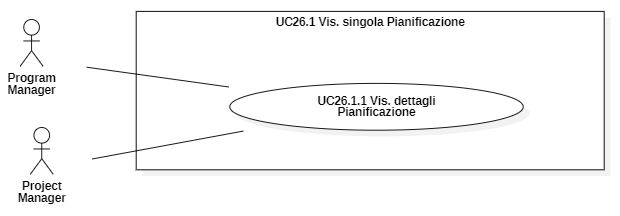
\includegraphics[width=0.75\linewidth]{usecase/UC26.1} 
    \caption{Caso d'Uso 26.1 espanso}
\end{figure}

\begin{itemize}[label=$\circ$]
\item \textbf{Attore:}  Project Manager o Program Manager;
\item \textbf{Descrizione:} il Project Manager o il Program Manager possono visualizzare la Pianificazione selezionata. Il Project Manager può vedere solo le Pianificazioni associate alle sue Richieste, mentre il Program Manager può vederle tutte;
\item \textbf{Precondizioni:} la lista delle Pianificazioni è visualizzabile;
\item \textbf{Postcondizioni:} la Pianificazione selezionata è visualizzabile dal Program Manager o dal Project Manager;
\item \textbf{Estensioni:} UC26.2;
\item \textbf{Inclusioni:} il caso d'uso non ha inclusioni.
\end{itemize}

\subsubsection*{UC26.1.1 - Vis. dettagli Pianificazione}
\begin{itemize}[label=$\circ$]
\item \textbf{Attore:}  Project Manager o Program Manager;
\item \textbf{Descrizione:} il Project Manager o il Program Manager possono visualizzare la
Pianificazione selezionata;
\item \textbf{Precondizioni:} la Pianificazione singola è visualizzabile;
\item \textbf{Postcondizioni:} il Project Manager e il Program Manager possono visualizzare
i campi di una Pianificazione selezionata;
\item \textbf{Estensioni:} il caso d'uso non ha estensioni;
\item \textbf{Inclusioni:} il caso d'uso non ha inclusioni.
\end{itemize}






\section{Tracciamento dei requisiti}


 

